\documentclass[a4paper,11pt,titlepage]{article}
\usepackage{graphicx}
\author{Abrie Greeff\\B.Sc Hons (Computer Science)\\Department of Computer Science\\University of Stellenbosch}
\title{Title}
\begin{document}
\maketitle
\tableofcontents

\section{Question 1}
% \begin{figure}[htbp]
%    \centering
%    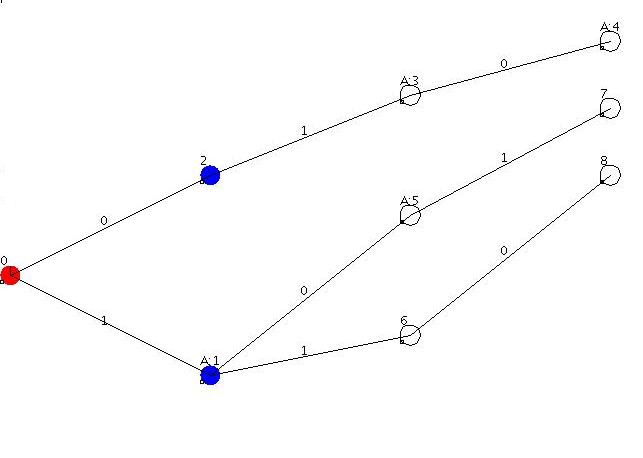
\includegraphics[width=7cm]{step1.png}
%    \caption{Hand designed DFA}
%    \label{Fig:dfa1}
% \end{figure}

\section{Question 2}


\begin{thebibliography}{9}
\bibitem{lang} D Harel,
\emph{On Visual Formalisms}, 
Communications of the ACM, Vol. 31 Nr. 5, 1988, pp 514-530

\bibitem{web1} 3D Studio Max,
\emph{Autodesk 3ds Max},	
[Online], Available from \emph{http://www.autodesk.com/3dsmax }

\bibitem{sipser} M Sipser,
\emph{Introduction to the Theory of Computation},
1997, p. 35


\end{thebibliography}
\end{document}
